
\section{Results}

\subsection{Predicting Performance on MED Dataset}

Figure \ref{fig:blb} displays the EERs of the video detection system on both the Kindred and MED data sets along with the BLB predicted standard deviations for each event. The average EERs for the Kindred and MED datasets are 36.1\% and 34.9\%, respectively. The average predicted standard deviation is 7.1\% and the average difference between event EERs for the Kindred and MED dataset in terms of predicted standard deviations for that event is .60. Although not all event EERs fall within 1 event standard deviation of each other, with the largest gap coming from event 6 with a 1.77 standard deviation gap, it appears that generally the performance on the MED dataset is reasonably bounded by the BLB's predictions. 

\begin{figure}[ht]
\centering
\subfigure[Events 6-15]{%
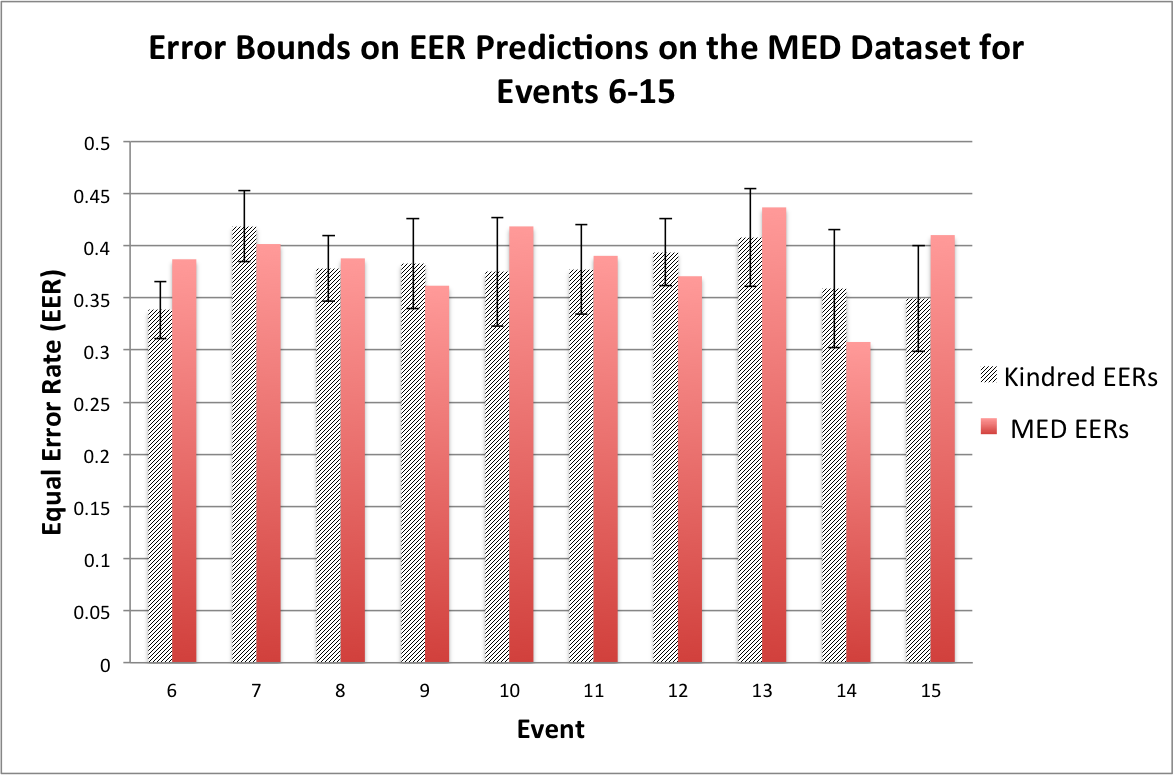
\epsfig{file=figures/errorbounds6-15.png, height=2.0 in, width=3.3in}
\label{fig:blb1}}
% \quad
\subfigure[Events 21-30]{%
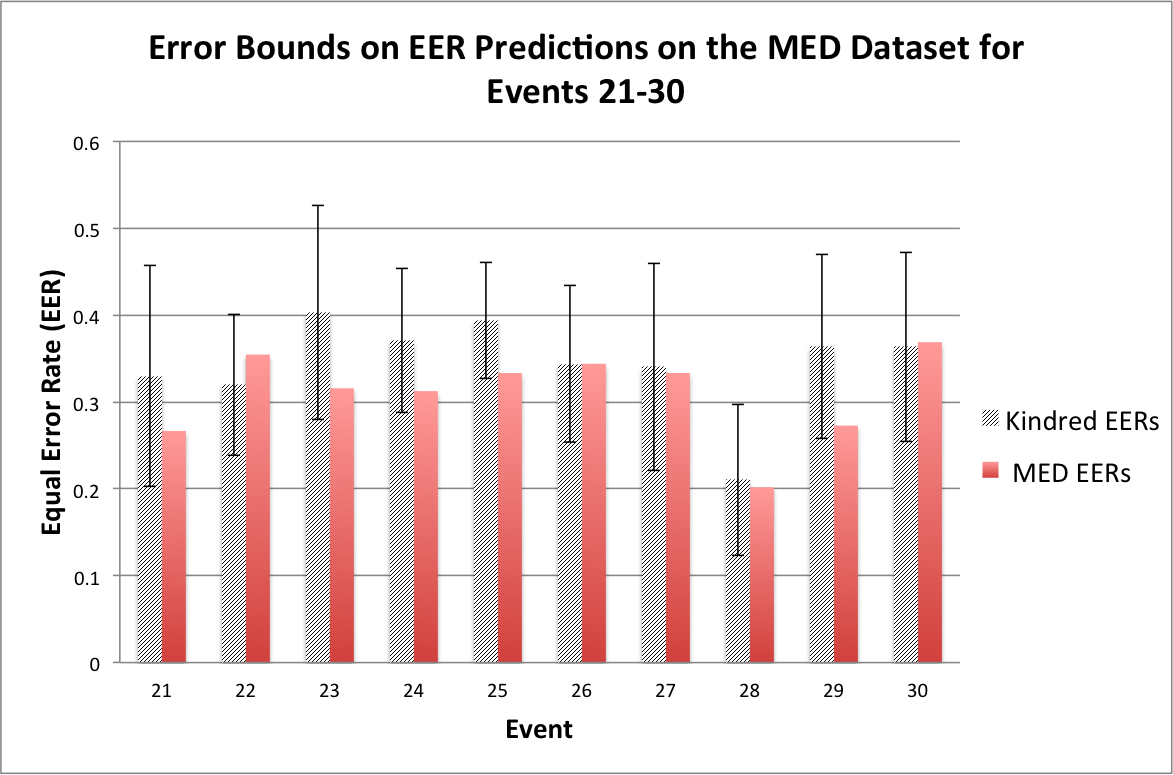
\epsfig{file=figures/errorbounds21-30.png, height=2.0 in, width=3.3in}
\label{fig:blb2}}
%
\caption{The performance of the video detection system on the Kindred and MED datasets. 
 The error bars display the BLB standard deviations that estimate the variance on the MED dataset from the performance on the Kindred dataset.}
\label{fig:blb}
\end{figure}


\subsection{Comparison to Na\"ive Python}


\begin{figure}
\centering
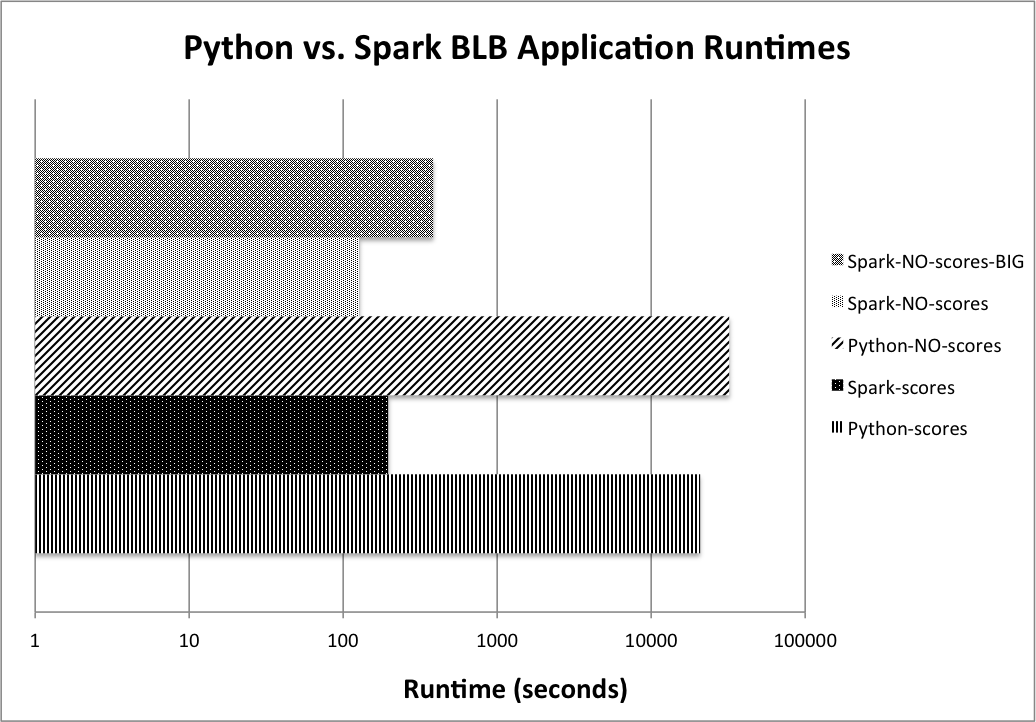
\epsfig{file=figures/pythoncompare.png, height=1.9in, width=3.3in}
\caption{Comparison of runtimes of native Python and generated Spark code. The Spark code, finishing in less than 7 minutes achieves more than a 2 order of magnitude speedup over the 5+ hour Python times. }
\label{fig:python}

\end{figure}
 

--table comparing times between distributed code and python for a few example runnings of blb  

or sideways bar chart showing times, with log scale axis  ?
